\documentclass{beamer}

\usepackage[main=english,finnish]{babel}
\usepackage{cmbright}
\usepackage{fontspec}
\usepackage{booktabs}
\usepackage{hyperref}
\usepackage{graphicx}
\usepackage{pifont}
\usepackage{layout}
\usepackage{tikz}
\usepackage{pgfplots}

\newcommand{\cmark}{\ding{51}}%
\newcommand{\xmark}{\ding{55}}%

\hypersetup{pdfencoding=auto}

\newsavebox{\mysavebox}
\newlength{\myrest}

%\usepackage{polyglossia}
\setsansfont[Ligatures = TeX,
             BoldFont  = CMU Bright SemiBold,
             ItalicFont = CMU Bright Oblique,
            ]{CMU Bright Roman}
\setmainfont[Ligatures = TeX,
             BoldFont  = CMU Bright SemiBold,
             ItalicFont = CMU Bright Oblique,
            ]{CMU Bright Roman}
\setmonofont[Ligatures = TeX,
             BoldFont  = CMU Typewriter Text Bold,
             ItalicFont = CMU Typewriter Text Oblique,
            ]{CMU Typewriter Text}
\usetheme{Madrid}

\mode<presentation>
\setbeamercovered{transparent}
\setbeamertemplate{enumerate items}[default]
\setbeamertemplate{itemize items}[default]

\title[Finnish language text mining]{Extraction, exploration and exploitation of diverse Finnish language texts}
\subtitle{TIES445 Data Mining project}
\author[Robertson, Kanushin \& Qing]{Frankie Robertson\inst{1} \and Max Kanushin\inst{2} \and Li Qing\inst{3}}
\institute[JYU, LETI, SWUFE]{\inst{1} University of Jyväskylä \and%
                      \inst{2} Saint Petersburg State Electrotechnical University \and%
                      \inst{3} South Western University of Finance and Economics
                    }

\date{18th of April, 2016}

\titlegraphic{
  
\includegraphics[height=1.5cm]{jyu.pdf}
  \hspace{1cm}
  
\includegraphics[height=1.5cm]{leti_logo.png}
}

\begin{document}

\section{Title}
\begin{frame}
  \titlepage{}
\end{frame}

\section{Contents}
\begin{frame}
\frametitle{Contents}
\begin{enumerate}
  \item Orientation and aims\pause{}
  \item Extraction (scraping + preprocessing)\pause{}
  \item Exploration (mainly visualisation through dimension reduction)\pause{}
  \item Exploitation (obtain metrics which could be useful for presentation directly to an end-user or for use within a larger application)
\end{enumerate}

\end{frame}

\section{Orientation \& aims}
\begin{frame}
\frametitle{Orientation}

\begin{itemize}
  \item The Finnish language is used in different ways in different contexts.\pause{}

  \item For Finnish in particular there is a marked difference between spoken and
        written Finnish.\pause{}

  \item There are more complex grammatical features of Finnish which are used
        only rarely (in particular many inflections are used only rarely).\pause{}

  \item Wouldn't it be nice to be able to distinguish between written and
        spoken and between less and more complex Finnish?
\end{itemize}

\end{frame}

\begin{frame}
\frametitle{Aims}

\begin{itemize}
  \item Create a data set which characterises the range of these two dimensions
        of Finnish. \textit{(Extraction)} \cmark{}\pause{}

  \item Create features based on this data set and visualise them.
        \textit{(Exploration)} \cmark{}\pause{}

  \item Create a model which can attempt to characterise unseen data.
        \textit{(Exploitation)} \xmark{} -- still at the ideas stage
\end{itemize}

\end{frame}

\section{Extraction}

\begin{frame}
  \frametitle{Sources}
  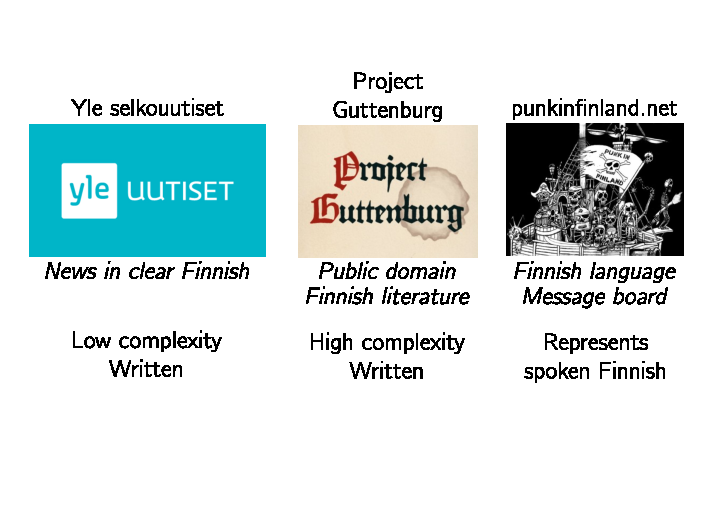
\includegraphics{sources.pdf}
\end{frame}

\begin{frame}
  \frametitle{Scraping \& data processing pipeline}
  \begin{columns}[onlytextwidth]
    \begin{column}{0.7\textwidth}
      \begin{itemize}
        \item We used Scrapy to write three custom spiders in Python. One key
          advantage of using Scrapy is that it makes it easy to write a reasonably
          well performing event based spider.\pause{}

        \item Another Python script converts the raw text into a series of
          matrices in a load'able .mat file using numpy \& scipy. The matrices
          are arranged in a similar way to the fisheriris data set.  Different
          features of the data are stored in different matrices...
      \end{itemize}
    \end{column}
      \begin{column}{0.3\textwidth}
      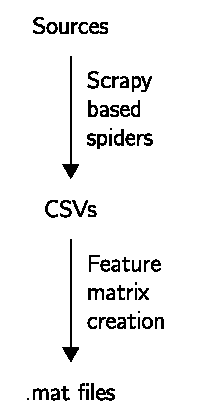
\includegraphics{pipeline.pdf}
    \end{column}
  \end{columns}
\end{frame}

\begin{frame}
  \frametitle{Preprocessing \& feature extraction}
  \begin{itemize}
    \item One set of matrices for distributions of word length and sentence
      length. Tokenisation using nltk.\pause{}

    \item Other matrices based on gramatical analysis using FinnPos, a
      morphological analyser and part of speech tagger (built on top of another
      project called OMorFi).\pause{}

    \item One matrix measures inflection complexity. It should be possible to
      segment word forms into morphs (and get distribution of morphs per word)
      but requires in depth fiddling with FinnPOS. For the sake of time just
      used different between lemma length and word form length.\pause{}

    \item Another set of matrices to represent part of speech distribution of
      individual words, pairs of words and and triplets of words (unigrams,
      bigrams, trigrams).
  \end{itemize}
\end{frame}

\begin{frame}
  \frametitle{Aside/soap box: the law}
  \begin{itemize}
    \item The legality of text mining on copyrighted material (which is pretty
      much everything recorded due to the Berne Convention) is unclear in the
      EU\pause{}

    \item In the US the recent Google Books case has cemented the the idea of a
      ``transformative factor'' of fair use (at least if you're Google)\pause{}

    \item Science Europe has published a detailed document about these issues:
      \href{http://www.scienceeurope.org/uploads/PublicDocumentsAndSpeeches/WGs_docs/SE_Briefing_Paper_textand_Data_web.pdf}%
      {Text and Data Mining and the Need for a Science-friendly EU Copyright Reform}\pause{}

    \item One of the recommendations is that research organisations should take a
      hands off approach and allow individual researchers to make their own
      choice as part of the process of pushing for new copyright exceptions
      rather than insisting on strict adherence to the obeying the letter of the
      law
  \end{itemize}
\end{frame}

\begin{frame}
  \frametitle{Exploration - dimension reduction on trigrams}
  \begin{itemize}
    \item Tooks a classwise sample of the trigrams\pause{}
    \item Computed multi dimensional scaling on 4 different distance measures (grid search)\pause{}
    \item Euclid vs cityblock distance and absolute trigram frequency versus frequency normalised for standard deviation
  \end{itemize}
\end{frame}

\begin{frame}
  \frametitle{Exploration - dimension reduction on trigrams}
  \begin{columns}[t]
    \begin{column}{0.5\textwidth}
      \vspace{-3em}
      % This file was created by matlab2tikz.
%
%The latest updates can be retrieved from
%  http://www.mathworks.com/matlabcentral/fileexchange/22022-matlab2tikz-matlab2tikz
%where you can also make suggestions and rate matlab2tikz.
%
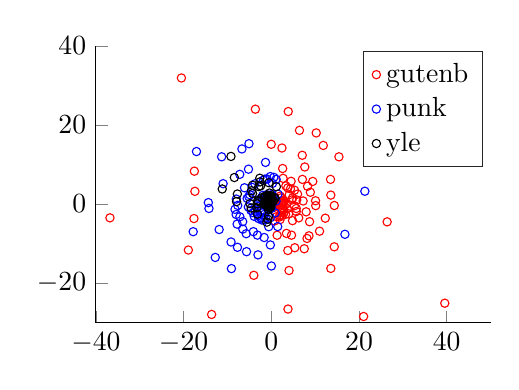
\begin{tikzpicture}

\begin{axis}[%
width=142.638pt,
height=100pt,
at={(0pt,0pt)},
scale only axis,
xmin=-40,
xmax=50,
ymin=-30,
ymax=40,
axis background/.style={fill=white},
axis x line*=bottom,
axis y line*=left,
legend style={legend cell align=left,align=left,draw=white!15!black}
]
\addplot[only marks,mark=o,mark options={},mark size=1.5000pt,color=red] plot table[row sep=crcr]{%
2.51853147043619	-0.184312717592451\\
8.26217619598809	4.47292959644027\\
10.1257095556266	-0.42447242519652\\
6.42438505277432	18.6082337925962\\
-17.6316402536924	-3.69296505700956\\
7.0541000442222	12.3053295525194\\
2.88091530229797	-2.23961846469056\\
-3.98661168122304	-18.0552568532048\\
2.03311363276535	1.97908696818103\\
4.83941574918701	-4.22374882770151\\
1.18794686601354	-3.22374105305984\\
10.0862392775687	0.805557345726814\\
13.5032455112578	6.2154040330835\\
2.91270514549044	-0.478899572580442\\
26.4132244609386	-4.52780370244988\\
-3.62962990178463	23.9683118574989\\
8.72901835980518	-4.49619167726029\\
15.4218899696225	11.9214253286328\\
5.98684780784645	2.48882516232038\\
3.86300840031335	23.3764740410342\\
2.68870304464699	6.47989311717792\\
13.5697220653633	-16.31090199832\\
3.65284065328639	-1.17477626071382\\
-17.5404875595048	8.28847647171796\\
11.844987560195	14.799809042523\\
12.308378310168	-3.61157568417828\\
1.32660032394358	-7.92086523901972\\
14.3640083238055	-0.393053670258017\\
6.24433054435604	-3.52618226397873\\
3.95107819885937	-2.4983135110463\\
2.17015513267978	1.50355353131717\\
-17.4177292854272	3.18871233920741\\
3.46660429466226	0.0109492572943127\\
2.48314639434509	-2.88556287806247\\
4.04365781087909	-16.8376475722159\\
3.75891306681309	4.05773368308417\\
5.26149095501228	-0.462263376080436\\
2.59003154937064	8.96316640089833\\
39.5532046980991	-25.1067104598263\\
0.407951201991969	0.02396407355619\\
0.831773952175422	-0.781444349770738\\
2.61818417043816	0.163957623908508\\
13.5691513906256	2.23916983237986\\
7.94458452904602	-1.9898946466416\\
5.79900293516835	1.00762412181527\\
5.69066523017537	-1.14923836753081\\
7.09257012448719	6.20962588075177\\
2.57579092179109	-1.70479568264114\\
3.77164114999401	-11.7780223057101\\
2.83644467661935	-1.42769989592304\\
3.2474181080797	-2.634607526441\\
3.80556891185842	-26.5833985519064\\
1.17667798947018	-0.130248483731058\\
8.14269288113947	-8.73325770201357\\
2.28077405263092	-2.20800051381286\\
7.2516260496715	0.750824735657847\\
4.08153585634343	2.32888172279958\\
0.319817504697377	-0.203626849993584\\
4.51007095511572	5.72806499709329\\
7.51443408665969	-11.3338689649879\\
-36.78975085484	-3.51472993046279\\
1.91430377811199	-3.2734494293099\\
5.69928565051815	-1.91737796909912\\
3.45232263701223	-7.45036103063757\\
2.77988951500069	0.69487832580603\\
0.547388075906283	-0.0654066620063768\\
0.0875673829841207	0.00217036591279903\\
0.521766899229599	-0.235481064485355\\
1.93792220755623	-2.90705161325516\\
-0.0195023831141549	15.0879342980139\\
4.60789828347238	-7.8994843206061\\
-13.6062525582758	-27.9514280940396\\
8.90438335671793	2.96413894472279\\
4.69225631037036	1.00482150404113\\
7.63411867961073	9.34898543210006\\
1.9902739825234	-3.95751492973122\\
44.8654538629269	30.0444692527788\\
9.45152567022065	5.69184092340858\\
2.0403827265701	0.318388140515972\\
2.58684057095892	0.479187780753699\\
8.5906902355994	-8.06468718707357\\
0.515177601872353	-0.164324785161728\\
-18.9118559677171	-11.6585612436391\\
14.3564511686899	-10.8424123317187\\
0.698012171515182	-0.364638750584768\\
-20.4948023555551	31.8618702731146\\
0.757921072570943	-4.30105326287514\\
23.0244869661186	13.492848280421\\
4.37027102098649	3.82366016763398\\
11.0009651319555	-6.890486120275\\
2.67940589462561	0.922996642161828\\
5.35091489358535	-11.077714860402\\
4.84837921416837	1.53587487442259\\
0.750731672477204	-0.685721267916706\\
3.31865504629004	4.56364959039762\\
21.0493949340569	-28.4682593946079\\
5.29815286773717	3.47728772793199\\
2.75617053727831	-1.10791181640944\\
2.43013284344304	14.1503125759873\\
10.2449134298631	17.9664276965797\\
};
\addlegendentry{gutenb};

\addplot[only marks,mark=o,mark options={},mark size=1.5000pt,color=blue] plot table[row sep=crcr]{%
-0.403980774776403	0.00328148580323619\\
-1.10282744241204	2.32008287646816\\
-0.206102261775647	-3.47537773602667\\
-0.463600284207872	-0.164803150658163\\
-0.417371688980129	0.0586183320875805\\
-4.91149436088287	2.342786178175\\
-4.64861467376553	-1.6165921455382\\
21.3330415079526	3.21457705956198\\
-4.36211693423882	4.18761453597828\\
-3.16367791323195	-7.88932956353823\\
1.08156622067417	0.731877298290645\\
-6.51605735545794	-4.48352537181294\\
-0.430737715572035	0.104139964795088\\
-1.31130854961834	10.5081505047129\\
-5.72198380492324	-7.52510554559928\\
-0.231991992815371	-1.04258172063041\\
-0.359541027712433	-0.0135788177040574\\
-0.596664298284556	-0.940922356785205\\
-0.312908485605029	0.0688664058401586\\
0.284644720805896	5.20675010185785\\
-2.36238544336484	-1.5873031368066\\
-2.11117034313714	-4.07260045129809\\
1.46147312457513	-5.72382320266239\\
-1.33686647355285	-0.49861679939844\\
-2.07214529606959	-1.71978779206716\\
-9.08921131288771	-16.3556549656435\\
-1.64386855585353	-2.66360070238936\\
-4.09171344060858	-7.01005426415341\\
0.0219159067818667	-15.6934624347684\\
-2.55985919475721	1.25261552379262\\
-2.42694427711311	-3.48498714938295\\
-1.6327566648236	-8.49277290282305\\
-7.97728590143031	1.23841583274833\\
-0.591797223966666	-5.76090787968029\\
0.206222310419974	2.40772690145041\\
0.0417539618313901	-1.10539731819445\\
-1.32813603342589	-3.60809846364411\\
-6.48783013158907	-6.36178661003021\\
-0.501217460647705	-0.0609983569093365\\
-1.087509630012	1.55632840624736\\
-1.79264898768127	6.01615292454608\\
-7.16737901583008	-3.23899704368259\\
-1.29140243508497	1.37159087125057\\
-6.10891709427246	4.08762334632099\\
-1.69382051170602	-3.96278709337816\\
-5.64595591121832	-12.0716886865255\\
1.10540015049015	6.21471010380721\\
-1.94512950599353	2.16815558597513\\
16.7863294435836	-7.67608672398011\\
-1.91281213300515	1.23939349936663\\
-3.04136607053091	-12.876928990509\\
-12.77973971829	-13.5295061098895\\
-5.12792656607323	1.8503126754849\\
-5.08894799183526	15.2428578189538\\
-8.01209234029149	-2.66700133776091\\
-9.17783838959989	-9.62548779163472\\
-2.95453434176836	-2.88728170439903\\
-4.15955458564796	-2.20793651132659\\
0.886142199176682	-2.26027060988823\\
-0.239079114469361	6.9277269327061\\
-0.379747516761049	0.0858577685427575\\
-2.87976558684443	0.286338673786173\\
-1.71866619820557	0.0124706938855573\\
-5.22905916580724	-0.770432947603014\\
-2.85407697340887	-3.71563145036348\\
-1.44486773173754	6.29760447337667\\
-11.3229583395489	11.9239282653846\\
-3.89159802496091	-3.13844547999634\\
-0.973165744665479	-0.957038690653725\\
-5.5086652676079	1.39803231409389\\
-2.03261055681692	-2.22417470345435\\
-7.79773783165797	-5.09991568260676\\
-7.19076232901107	7.48395929555837\\
-6.69861423345436	13.9078631895695\\
-3.74702931094532	5.086821857335\\
0.550450904701844	1.07334741328696\\
-1.0503295353588	-0.625828565703845\\
-0.642830248512067	-0.183848501331205\\
-0.954355175534723	6.29776941964887\\
-0.512427938676299	2.16360741422897\\
-7.71518183502221	-10.9669274566249\\
-0.417378836865991	0.0586251595148182\\
-2.86075805897662	-0.512183223947271\\
1.52365935527504	2.48702432472486\\
-3.60198200287495	-1.82190512317603\\
-8.27628641589878	-1.35628146785225\\
-14.3591391384162	0.338375533779831\\
-11.8889455659653	-6.47253054145387\\
-0.463847696521288	-0.694034331673034\\
-0.470624884955838	-0.322868577308096\\
-1.68211782013982	0.502516803308894\\
0.577593554526893	6.72918972604184\\
-0.322760374506226	-1.21601552274306\\
-10.9900799182404	5.12952909323946\\
-5.19962408906541	8.79494930172432\\
-7.65566103522514	-0.36138722472356\\
-14.2142594432158	-1.14037570427171\\
-17.8087871132628	-7.01942382239635\\
-17.057893584273	13.2549732597122\\
-0.212048833445057	-10.3722208125025\\
};
\addlegendentry{punk};

\addplot[only marks,mark=o,mark options={},mark size=1.5000pt,color=black] plot table[row sep=crcr]{%
-0.328654801878857	-0.0500543375326982\\
-4.86266674273164	0.0795317326340382\\
-0.337151640896567	0.209873851445664\\
-0.330605634188824	0.1432821447718\\
-3.24634309431319	0.00803190834655348\\
-1.38379678487107	0.586560048210144\\
-0.67350572554797	0.742643419183227\\
-0.00647992821046443	0.0376321542936072\\
1.15836673929671	4.35890261700122\\
-0.168723537736775	0.0507298697261175\\
-4.5085187391032	3.34030608587631\\
-0.321699479204819	-0.0605443872560003\\
-2.84826323019707	4.38705446493945\\
-0.378263364459288	0.00829536585402984\\
-0.406880244212181	0.0928289281513506\\
-0.165107256237315	-0.0119656953134297\\
-1.32883604065862	1.94940219814624\\
-0.422600602266007	0.214751890324794\\
-2.44120364416916	4.57056691211961\\
-0.394852563635669	2.75784912215863\\
-0.64392423064305	-0.353496246269523\\
-0.34909908924777	-0.0222332545238257\\
-2.62833477477046	6.50799287296493\\
-0.374951356346824	-0.112773754292264\\
-3.09256901488895	0.870034434303233\\
-0.346092268474915	-0.0804909903035103\\
0.448348613597455	0.717572298222559\\
-0.386551777378023	0.166509461572129\\
0.69197311045491	1.59973913099466\\
-2.58153152223869	5.57957291008154\\
-0.141233244029803	2.11388731148648\\
-3.30497125937077	-0.964893024025196\\
-1.1786201219409	0.342487910092368\\
-0.807969301020379	-0.188090271240943\\
-0.195672659039224	-0.841302406153312\\
-0.559433281125515	1.63293213962153\\
-0.115733674577238	1.41241031001021\\
-0.832798761820308	-0.431950514037451\\
-0.338008050942712	-0.0708420679048541\\
-0.339555653530237	0.167626020247231\\
-4.58538207951765	-1.03087767047636\\
-0.39145063032325	-0.0705087263593928\\
-0.15930762529193	0.0651699666680513\\
-2.95348114147617	0.621239353692886\\
0.0699650135215779	0.67508899075367\\
-0.248991191014286	0.149763067018812\\
-7.92641027347811	0.595643386437624\\
-11.1885356906248	3.78212671863224\\
-0.369964005843769	0.0181647458148593\\
-0.393387349879404	0.0461055365641759\\
-0.0720022056712163	-0.551647789100887\\
-1.44438387040573	-0.203557739638604\\
-0.545801218898761	5.36108809417012\\
-1.23310747247467	0.0587986002185468\\
-0.262277967949984	0.144265892685776\\
-0.860446796389882	2.20671063099258\\
-0.373241536841267	-0.0538429498671379\\
0.876991513881362	1.46225097067802\\
-1.00306434748136	-4.59686974462478\\
-0.365721902066377	0.175479590402377\\
-1.02646935852601	0.668908617853316\\
-0.338174625834035	0.0284826751035305\\
-7.73198431044862	2.5155016942081\\
-0.302611853437675	0.0833202291082351\\
-1.60664294416758	1.81558453260687\\
-0.634543438286863	-1.43693459824167\\
0.17352132350327	1.45546701835008\\
-0.282774013592953	0.0529746694401281\\
-0.244651694586423	-0.382810233198804\\
-0.399383281677744	0.0511999308641325\\
-1.33993508204964	0.995356471208997\\
-0.392678461088791	0.156291512913734\\
-4.26357737826278	2.66892325297902\\
-0.381180678473136	0.184077248247114\\
-0.32525966846231	-0.0405529095652741\\
-0.624146574171529	-3.03583677470401\\
-0.259897376914424	1.19061325646941\\
-0.248624883603136	0.10963543737445\\
-0.824568466507032	-0.697578271257888\\
-0.385950142806811	-0.244172925360417\\
-0.3479723639226	1.91008384548529\\
-0.668639691013584	-0.837133236654274\\
-0.389264728864348	0.0673013869014663\\
-0.398332146621786	-0.486868662065956\\
-1.14942126674475	-0.261304834336703\\
-0.375056434518098	0.0984596186197012\\
-0.426534888571467	0.152086335224707\\
-0.244359807185439	0.129959590267436\\
-9.19687300275266	12.0178147459155\\
-0.441744659360316	0.0097820035267108\\
-0.383941745642254	0.113206937372928\\
-0.623450512467752	-0.584827830713087\\
-0.236710294131738	-0.48499948252646\\
-2.15696386647133	1.58288104060005\\
-0.727954297968883	1.21447050441385\\
-8.42824697289685	6.67916325470418\\
-3.14961271482201	-2.56922594084954\\
-0.785411905427629	-3.86773872426319\\
-4.28385891196915	4.72569334273723\\
-0.191174710291028	0.0450517711183585\\
};
\addlegendentry{yle};

\end{axis}
\end{tikzpicture}%
      \vspace{-3.5em}
      % This file was created by matlab2tikz.
%
%The latest updates can be retrieved from
%  http://www.mathworks.com/matlabcentral/fileexchange/22022-matlab2tikz-matlab2tikz
%where you can also make suggestions and rate matlab2tikz.
%
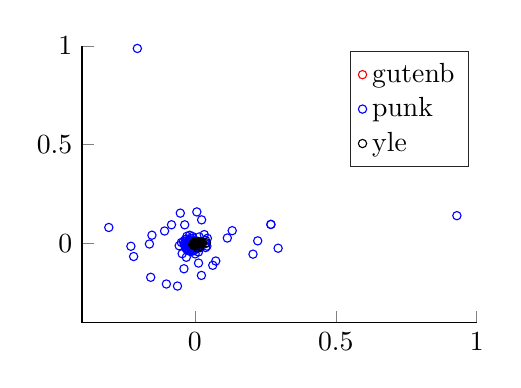
\begin{tikzpicture}

\begin{axis}[%
width=142.638pt,
height=100pt,
at={(0pt,0pt)},
scale only axis,
xmin=-0.4,
xmax=1,
ymin=-0.4,
ymax=1,
axis background/.style={fill=white},
axis x line*=bottom,
axis y line*=left,
legend style={legend cell align=left,align=left,draw=white!15!black}
]
\addplot[only marks,mark=o,mark options={},mark size=1.5000pt,color=red] plot table[row sep=crcr]{%
-0.00436542813205768	-0.00386574006000168\\
-0.00394570448899721	-0.0036873630406982\\
-0.00371254716991265	-0.00395510153179676\\
-0.00423310813644724	-0.00251099733755494\\
-0.00280909753137377	-0.00312285891258345\\
-0.00430464773124558	-0.00367572312864427\\
-0.00466355117712597	-0.00378595132380166\\
-0.00317582028752623	-0.00343613279729958\\
-0.00717461422826419	-0.00316619690518935\\
-0.00414907411110264	-0.00370455353714345\\
-0.00423064673450498	-0.00305781131350245\\
-0.00486204868540564	-0.00250472158671116\\
-0.00515668778048111	-0.00307113926646871\\
-0.00456494183799222	-0.0027233791091295\\
-0.00330831572664715	-0.00127700852488018\\
-0.00444467414761741	-0.00384142281149707\\
-0.00246226370861329	-0.003835171345609\\
-0.00289708004730083	-0.00212277504915931\\
-0.00395215898055054	-0.00324264223524448\\
-0.00300560084998987	-0.00275139660960528\\
-0.00231394807452546	-0.0029528579323623\\
-0.00507917507064932	-0.00351935349143805\\
-0.00484253476510236	-0.00387534499168193\\
-0.00476882957773839	-0.00388066451038783\\
-0.0033279468540786	-0.0032925487008874\\
-0.00273570138367955	-0.00206751865515516\\
-0.00531487419731184	-0.00388035447410111\\
-0.00469419247276828	-0.00400645963266594\\
-0.0036648963310752	-0.00330364785753154\\
-0.00502619856494359	-0.00470896508251025\\
-0.00399162505794104	-0.00320776360331094\\
-0.00359229865368105	-0.00349531357814315\\
-0.00452220964200991	-0.00357751090119253\\
-0.00311092448522061	-0.00315132223042905\\
-0.00370524911091882	-0.00296851283855095\\
-0.00470087466357958	-0.00302270992499597\\
-0.00378362056125467	-0.00347429721647659\\
-0.0154478089199347	0.0244624753411588\\
-0.00382392112864079	-0.00267566387275731\\
-0.00299265346408865	-0.00327866581563134\\
-0.00161873950681449	-0.00270090424620082\\
-0.00389817582526509	-0.00280711667493061\\
-0.00334887774598823	-0.00366815501506621\\
-0.00456690116818679	-0.00318791821558983\\
-0.00342268841850307	-0.00308061059650877\\
-0.0048909947597987	-0.00357538789304515\\
-0.0052212340470522	-0.00366123565278773\\
-0.00274733285026572	-0.0031193406486319\\
-0.00111040324460094	-0.00227199996397341\\
-0.00386226998223864	-0.00334027039684826\\
-0.00413583511672526	-0.00362474753891494\\
-0.00305801032413154	-0.00300629899218309\\
-0.00505392802122561	-0.00485694233190198\\
-0.00349359580525897	-0.00320305517521138\\
-0.00344275760419365	-0.00302866347352615\\
-0.00327568215931436	-0.00345766096691162\\
-0.00408837267733391	-0.00333254895925367\\
-0.00441660540342165	-0.00252127391434924\\
-0.00312794038217308	-0.00352297946427205\\
-0.00424982108672018	-0.00373904450357508\\
-0.00339519867398191	-0.002252378628769\\
-0.00456312911617388	-0.00341147001715025\\
-0.00337498939653525	-0.00333242922517188\\
-0.00680236095330191	-0.00262582230657433\\
-0.00334068724818006	-0.00357922017715662\\
-0.00611273105146214	-0.00263547825662739\\
-0.00566840848319101	-0.00434839135185966\\
-0.00318764893659183	-0.00325650030460015\\
-0.00442843251636863	-0.00329084744926718\\
-0.00434023437137321	-0.00293269432886813\\
-0.00360429251375093	-0.00322474721855117\\
-0.00436613894847938	-0.0034646114208158\\
-0.00618216001293664	-0.0023481680716228\\
-0.00376461669403101	-0.0031472432528717\\
-0.00442067704159426	-0.00371464377566551\\
-0.00368682251583553	-0.00382452663368465\\
-0.00251619395873623	-0.00229849707184773\\
-0.00496355105425818	-0.00432223050819019\\
-0.000813499539406579	-0.00626226179369645\\
-0.0034545773907607	-0.00365339226261715\\
-0.00419597452761459	-0.00350902674885943\\
-0.00418427064133549	-0.00347910284563425\\
-0.00318698110062347	-0.00339842799093333\\
-0.00404830519485456	-0.00281420115398269\\
-0.00342190935956772	-0.00351251537980963\\
-0.00401595953718831	-0.00357260553035951\\
-0.00387576142089008	-0.000118686568146038\\
-0.00321817132058919	-0.00215550740717629\\
-0.00439533399129689	-0.00345086889190142\\
-0.00492045828901406	-0.00335221130852252\\
-0.0036055265358812	-0.00359560791112651\\
-0.00249318268321514	-0.00327314664449374\\
-0.00458249287924039	-0.00378301707463185\\
-0.00299024874181149	-0.00254834207628452\\
-0.00461098529547099	-0.00333909826736765\\
-0.00338554235570986	-0.0023122342966127\\
-0.0053978105076117	-0.00364702598893329\\
-0.00360505866392979	-0.00280182223166513\\
-0.00301183162771011	-0.00340896917820721\\
-0.00364940614131526	-0.00362579861152802\\
};
\addlegendentry{gutenb};

\addplot[only marks,mark=o,mark options={},mark size=1.5000pt,color=blue] plot table[row sep=crcr]{%
0.929487083494097	0.140783389783946\\
0.0445796589845227	0.0261537196959803\\
-0.0283655990468501	0.000739798325236251\\
-0.203846399013863	0.986688359284883\\
0.26976884305596	0.0963992758389156\\
-0.0324153236463496	-0.0228534139045108\\
0.038270039939078	0.0159422180918408\\
-0.00805845526299033	-0.00420572248571644\\
-0.0143630574537353	-0.0153331399190636\\
-0.0133812288743156	-0.0409790228614054\\
-0.00770273688694869	0.0134059100422255\\
-0.0385370521174295	-0.127847192848491\\
0.295453433598767	-0.0240146466185428\\
-0.00669376911179568	-0.00280040423051986\\
-0.0199214729013329	0.00109831085234941\\
-0.013624805307249	-0.00260355317902403\\
0.115326420384981	0.0275841167508857\\
-0.305106135685608	0.0810241903217168\\
0.00806797500135062	0.00986947062655267\\
-0.0476625580614101	0.00510039507194406\\
-0.0275404158116708	-0.00556015132070534\\
-0.0085938092006303	0.0355988796707088\\
-0.00129633295890577	-0.0133541387952506\\
-0.0615144444023056	-0.215294592926458\\
0.0240934673788117	0.119539704271407\\
-0.0273432040806352	-0.0328293808308974\\
0.0234371294640465	-0.161611262715544\\
-0.0195893101323978	-0.00375997292437308\\
-0.0103350005358045	-0.00636865442439433\\
-0.107293725899414	0.0631209680695923\\
0.0636322392579717	-0.11036609111547\\
-0.00349800734582324	0.0138533013841359\\
-0.0136443229733535	-0.0180312789285906\\
-0.0158973535652893	-0.00878495621261766\\
-0.0120591042500185	-0.0134606072198521\\
-0.216938114458032	-0.0659834263604936\\
-0.0404932241544313	0.0105247882382644\\
-0.0146441300085366	0.00441740854249712\\
-0.0359084766356514	-0.00807362934649574\\
0.00182123111789556	-0.0280451519189013\\
0.01282264911591	-0.042920335367007\\
-0.0202485655347316	0.0118361531601573\\
0.132626875758369	0.0647801845041243\\
0.0376205688509029	-0.00102498700870106\\
-0.0295158664439007	-0.0251946009376094\\
-0.0213996322252551	-0.0139502126322865\\
-0.00321939929726247	-0.0124068549043526\\
-0.0358541573916265	0.0944612224009639\\
-0.00710624323186176	-0.0298519404397764\\
-0.100808848047388	-0.205008417539508\\
-0.0115802282493814	-0.0237162372603569\\
-0.0137912968235638	-0.0341218175433298\\
0.00717230658506105	0.159654133863922\\
-0.0343286472568597	-0.0122891014213705\\
0.00134311906593281	-0.014998322479853\\
-0.00554870025432436	0.0263420498678039\\
0.0131634639377794	-0.0991504153114955\\
0.042823544279218	-0.0132295498654316\\
-0.00594568097527994	-0.00289131042015343\\
-0.0276536756280367	0.00199263710059935\\
0.223072418115969	0.0133052238872818\\
-0.226728950547376	-0.0141187907859525\\
-0.152055138376358	0.0418653758083117\\
-0.156458203068412	-0.171004753082128\\
-0.0202951987890554	0.0162358517665257\\
0.00110313709860325	-0.0525313451560633\\
-0.0204839968282163	-0.00888599018981907\\
-0.0104941319960953	-0.00397932558559126\\
-0.0101132636240395	0.00699452837286434\\
-0.0280469771039833	0.0364420642296777\\
0.0189895615520099	-0.0214967244342006\\
-0.0100977354381736	0.000111219208181586\\
-0.00336890990431203	-0.0367046676795019\\
-0.0337538686019302	0.0202393322030603\\
0.0334160650236754	0.0448679298230225\\
0.0742721924905964	-0.0886605994704855\\
-0.0302064789272105	-0.0698729437275451\\
-0.0201306991436228	0.00369852813910251\\
-0.0553692711060648	-0.0116296188060872\\
-0.0826743676200707	0.0946894843753015\\
-0.00899199991248356	-0.0104594698290821\\
0.269751343384348	0.0964460121803725\\
-0.0229063371346631	-0.0365184705653947\\
-0.00386957347449317	-0.00213463064960002\\
-0.00672955367619698	-0.00776417385190491\\
0.0157068975033501	0.0329281959908874\\
-0.0449320115376977	-0.0515954034132112\\
-0.0182665709934882	0.0416585096371882\\
0.0385794237306297	-0.0204500762577657\\
0.206341054793833	-0.053982756646486\\
-0.020579119519987	-0.0255427362404663\\
-0.0117472938961797	-0.00141422829185554\\
-0.160955353955726	-0.00265130971445367\\
-0.0283692071643086	0.0122458203593213\\
-0.0143594494354506	-0.00549129619632431\\
-0.0514980628461361	0.153473414080716\\
-0.00653810823807234	-0.00377663016268377\\
-0.0287398253455823	0.0228567164609873\\
-0.0377768082780254	-0.00253995281365301\\
-0.0129427168466081	-0.00536238122743023\\
};
\addlegendentry{punk};

\addplot[only marks,mark=o,mark options={},mark size=1.5000pt,color=black] plot table[row sep=crcr]{%
0.00115819761499369	-0.00474370149396125\\
0.00242383921215567	-0.00119860004504164\\
0.00551247953471419	-0.00198784115973183\\
0.00265192019323283	0.00139212039782671\\
0.00507197499579378	-0.00380010048783183\\
0.00363767382645993	-0.0027685546559439\\
0.00458489924136314	-0.00208770253400988\\
-0.00182086978206762	-0.000626007377105226\\
0.000446458410493692	-0.00545591376828855\\
0.000784686008636069	-0.00293103229517371\\
0.00756703463733045	0.00521688091224602\\
0.000236958904481711	-0.0030349540764108\\
0.00339025975320601	0.00249597385903728\\
0.000345558982403572	-0.0040045018680819\\
0.00345693074946672	-0.00863391707198318\\
0.000563678182552586	-0.000896675500460152\\
0.00667829467445214	0.00227207130247829\\
-0.00157280222660394	-0.00639385753762209\\
0.013008149291044	-0.000378162991273987\\
-0.0035786692723901	-0.00565358296546354\\
0.00435499065963994	-0.00187961402694816\\
0.0105955124378951	0.00346067359848528\\
0.00221957317562089	-0.00555286842012214\\
0.0232135553204648	0.00220310753940827\\
0.00083775811169805	0.00217382778562745\\
0.000776863361479401	-0.00148991368496099\\
0.00728310309477306	-0.00126138840550338\\
0.019420162920767	-0.000129437642831838\\
0.00532477993682465	0.000956712243131921\\
0.000365963242202038	-0.00355121999566866\\
-0.00420112880013994	-0.00787169884951242\\
0.0171240938963838	-0.0145476609613345\\
-0.000998900369821102	0.00421116580263303\\
0.00693453632009358	-0.00314978008226212\\
-0.002568455403867	-0.00593519270237419\\
0.0109734896734373	-0.022266862094231\\
0.0219604538078827	0.00817211714147621\\
-0.00105873949106895	0.00274118098011096\\
0.00407478576822658	-0.000677117235668313\\
0.00370130877514431	-0.00110675543337342\\
0.0189733916054238	-0.0128199508437141\\
0.00156559885451558	-0.00125585685121899\\
-0.00178540131781155	-0.00433573549670481\\
0.00623506081320627	4.63421841069461e-05\\
0.00130829435706557	-0.00188726565946293\\
-0.00232429315725134	0.00354007005524679\\
0.00648513688269906	-0.00383540060173752\\
-0.000315903775102209	0.0016580377087884\\
0.00357859952677507	0.000543968050106351\\
0.0410005154107459	0.0039227121932364\\
0.00345920843385857	-0.00257807846424378\\
0.00462947866320411	-0.00290601174783371\\
0.000357541474266199	-0.005190138715644\\
0.0181660262142415	0.00252914101642738\\
-0.00577325271130851	-0.006578552379682\\
0.00532653997935728	0.000623387689916844\\
0.00249319283701492	-0.00418760665097496\\
-0.00744500482844592	-0.00547163617350012\\
0.00412026536092682	-0.00509465134661491\\
0.0021508202980916	-0.00199070819085272\\
0.00904648128096121	-0.00666448976344627\\
0.00266742979299185	0.000860761570167381\\
0.000276616441083452	0.000718590643236536\\
0.00281528875515766	-0.00512732437527794\\
0.00297837928597592	0.000621492561762334\\
-0.00237512315438725	-0.00185302516291297\\
0.00510582553504882	-0.000486011930158508\\
-0.00181743650472224	-0.00571496677469214\\
0.00101044635055645	0.000614583643829249\\
0.000270432114386672	-0.00226837177923497\\
0.00535425646091486	-0.00610293163298113\\
0.00375167692447827	-0.00661209111401456\\
-0.000888905001886977	-0.00106705181377361\\
0.00394291570245756	0.000194960012152142\\
0.00925487967666063	0.00366404724990177\\
-0.00206832725934817	-0.000890484659404399\\
0.00708331165804899	-0.00679836258119119\\
0.00331225375674817	0.00443012928086619\\
0.00517187586471745	-0.00122058557580555\\
0.0152741482603412	0.00261132248402423\\
0.009622902043814	-0.00317639025283122\\
-0.000125921743482866	-0.00293700408621482\\
0.0281582511460416	0.00313272509444438\\
0.00203427245840074	0.00145339336213104\\
0.00546861517133959	0.00494489010074475\\
0.00657278663407969	0.00104323411468061\\
0.00419675137847765	-0.00275007072060806\\
0.00492257253538553	-0.00255318426325067\\
-0.00237583196122454	-0.00628909610639129\\
0.0145631294571005	0.000605163259126259\\
0.00625632548152295	-0.00209296010616179\\
0.0107927938611533	-0.000641429006241036\\
0.0119481226773816	0.0103324407088792\\
0.00673085435573062	-0.000902311592440894\\
0.0152099570427786	-0.00111456806483046\\
-0.00269177407658434	-0.00912225430127991\\
0.00155261323120509	-0.00319333824895925\\
-0.0029892797732484	-0.00520036910313011\\
7.9438586940862e-06	0.00856944657153089\\
-0.00143291066764949	-0.00397280172335842\\
};
\addlegendentry{yle};

\end{axis}
\end{tikzpicture}%
    \end{column}
    \begin{column}{0.5\textwidth}
      \vspace{-3em}
      % This file was created by matlab2tikz.
%
%The latest updates can be retrieved from
%  http://www.mathworks.com/matlabcentral/fileexchange/22022-matlab2tikz-matlab2tikz
%where you can also make suggestions and rate matlab2tikz.
%
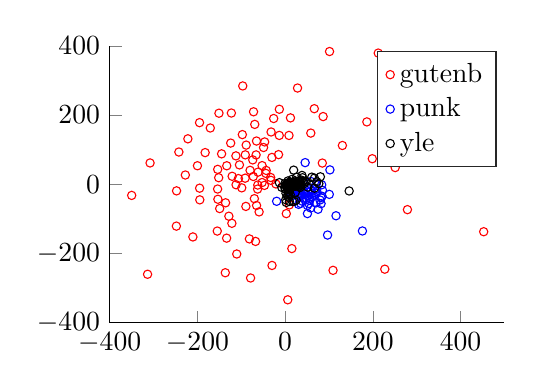
\begin{tikzpicture}

\begin{axis}[%
width=142.638pt,
height=100pt,
at={(0pt,0pt)},
scale only axis,
xmin=-400,
xmax=500,
ymin=-400,
ymax=400,
axis background/.style={fill=white},
axis x line*=bottom,
axis y line*=left,
legend style={legend cell align=left,align=left,draw=white!15!black}
]
\addplot[only marks,mark=o,mark options={},mark size=1.5000pt,color=red] plot table[row sep=crcr]{%
-133.150426194405	53.2755879024924\\
-69.2785037514332	172.84114972874\\
-194.585117363511	-45.2922230276321\\
273.924348782654	133.968436184656\\
-29.9450483071144	-234.979687280936\\
-242.290826570035	92.978778086212\\
-151.493244690336	18.7364055296434\\
86.6119624509559	195.431008661487\\
-47.2244224667956	-3.46443964823135\\
12.1452775703029	191.674872873159\\
-62.4363569430422	-2.50719327809267\\
-199.934030306199	53.2824906424347\\
-122.581326463517	205.676972813629\\
-120.8141726226	22.8378977284848\\
278.849893842278	-73.6289238497083\\
-78.8033246792294	-271.174918711882\\
2.62779491615774	-85.0802613132865\\
250.926035463601	48.0171031593571\\
-124.165768919251	118.819485279152\\
109.201201304914	-249.087984848646\\
-59.3733340448671	-80.1065338337041\\
-307.982454870409	61.4001757364528\\
-153.981791372708	-14.0246223479524\\
-210.346628802271	-152.499807456617\\
28.2587794749176	277.950176085223\\
198.681999631996	73.6146484607985\\
-13.4159033327852	140.968476122285\\
-221.784000787809	131.130913068244\\
-121.471542938873	-113.130156735267\\
-70.1730128477667	-41.8711066786164\\
-15.020205310003	85.4539924793027\\
-133.400005907028	-156.030706356161\\
-153.77758628153	42.8470190954763\\
-98.9200143263539	-10.5937313362558\\
-154.79370171866	-135.537325645442\\
-104.163805658639	55.7729305354928\\
-65.2937727616651	124.75117326414\\
84.8002691066802	61.0548854313286\\
212.273412124796	378.957094541162\\
-43.222544489262	39.7214137024363\\
-52.4857493165509	4.76646873309731\\
-46.6927007846332	122.104860413026\\
-96.6553178761392	283.976929701271\\
-170.671253721483	162.408909626457\\
-32.0733450362858	150.901677808185\\
-227.530239305654	26.5074972965701\\
-150.893556198424	205.169487306822\\
-73.8639548582893	70.2519566634575\\
130.536882854279	111.851975604898\\
-88.8190090676341	112.989205828453\\
-66.2479837746219	84.63194646381\\
5.98279188549946	-334.212457132882\\
-62.8169043903511	-14.1097844022182\\
-248.009379615692	-121.247421622868\\
-91.1916544776117	17.3312719521892\\
-72.0382581379764	209.286068291386\\
-153.351386719806	-43.5959578475939\\
-32.2801899419202	11.0423134374113\\
8.78944044138066	140.920152518926\\
-247.569226647742	-19.3086574960406\\
227.225814775088	-245.725064446878\\
-106.569259632201	16.2324367402265\\
-111.940916985338	-1.64804437042069\\
-89.5196092544592	-64.2599519216275\\
-112.205357209484	81.8518125312173\\
-43.7813151495365	31.1080466423783\\
-21.0093015429462	0.634442803946992\\
-72.6113638185692	22.2068763979843\\
-79.9625797100697	40.0107105911355\\
66.4750745501339	218.212888814978\\
-128.295216947246	-92.6248284474007\\
-349.866858964486	-32.4424809518971\\
-67.4094171404482	-165.478871661567\\
-81.4931068055192	-158.199525309895\\
-13.2277729804328	216.588505319995\\
-30.1166266151421	77.3439266137318\\
452.735460325781	-137.414016519392\\
-194.958255670906	-11.5499966979268\\
-65.1025936002555	-61.5654423483931\\
-90.9132918440723	84.7862720699132\\
-149.202529446632	-70.4832147138994\\
-61.7880279138889	34.824863952517\\
-136.424925319703	-256.020080198464\\
186.333348978127	180.050714990472\\
-52.5581588295026	53.6836742181479\\
-313.668606386821	-260.397488605149\\
9.61671142952462	-59.875571618308\\
248.081778600952	237.573382224154\\
-97.5864292321053	143.312253353189\\
15.2942737963658	-186.13227834412\\
-49.2238089164192	106.018018655419\\
-110.336824602819	-201.814827444785\\
-144.87864814121	87.7098113274974\\
-33.0267095331163	19.4417900862767\\
58.50665291466	147.707258823215\\
101.243509874995	383.499387360318\\
-182.390091032586	91.2837813140114\\
-135.791498474237	-53.8058862802919\\
-26.115621605554	189.851967792741\\
-195.179410760841	177.884352161417\\
};
\addlegendentry{gutenb};

\addplot[only marks,mark=o,mark options={},mark size=1.5000pt,color=blue] plot table[row sep=crcr]{%
9.7144218615479	-5.64042558857243\\
14.879877213618	-12.6648627518932\\
29.6968292049908	-31.1906543098371\\
10.0909179225287	-6.10423681901613\\
10.2060710130448	-5.91924509045843\\
29.8552072279136	-26.5453175160431\\
21.6187432647825	-17.7427106575075\\
176.232076660497	-135.25422163978\\
38.488816735732	-48.7175625884009\\
39.4135724822591	-31.8230231655081\\
12.5229047901871	-22.652310287075\\
19.8401095162094	-14.0646447305212\\
10.4764334045987	-6.02068619309365\\
102.091368838854	41.3770577139379\\
54.1588316750511	-55.7059959611792\\
18.1951338886704	-32.4525437892412\\
10.5199039540821	-6.1820998007367\\
10.8014383830684	-6.75271309595608\\
12.0077085080054	-8.58558466998209\\
21.999241661023	-20.3692164449304\\
33.8537113932995	-16.6618476685724\\
22.3296970527251	-11.986899799708\\
35.4631952198077	-55.6393368232389\\
12.2984255378585	-6.97798686529922\\
14.1890606732295	-10.2544610094762\\
84.0712813126647	-34.915734528905\\
14.22669712368	-9.56809589392574\\
60.1453189913376	-37.0104281937239\\
116.013141840365	-91.2705539976189\\
13.61264903013	-9.299628617893\\
14.7475325714956	-11.0587709040011\\
47.0852922002835	-45.4522453617703\\
55.1316821832458	-41.1802812100431\\
44.7566897163989	-40.559643891041\\
38.21715179377	-7.29185934859829\\
11.5544387505444	-7.08744233098934\\
17.3750699724941	-17.5464778411682\\
71.1134038309309	-26.3491928555662\\
15.3076700730963	-8.07421657140706\\
19.2121322972394	-9.12338908518113\\
27.2604142060388	-22.1705803080365\\
47.0034077131136	-16.7575415139406\\
13.4652361255897	-7.31092728722145\\
30.4515990388653	-12.853672398831\\
30.304843518207	-16.4083200356719\\
56.1169322567589	-47.0356456079352\\
70.6535657960706	0.13998644594115\\
16.933196251926	-10.0597852915722\\
100.658087143355	-29.4658138141737\\
12.4971095637539	-7.94192042468557\\
81.8091925642735	-38.7987424734625\\
58.1961588610053	-68.7578341539053\\
15.9247400564224	-10.301409209066\\
72.1776251723662	-21.35675867667\\
69.3295071099948	-15.1769179071561\\
50.7723428326136	-61.6716107431796\\
19.5416338357618	-10.1117563254102\\
21.473188198346	-8.80231484343127\\
-19.3788465230093	-49.4201846469268\\
34.8988495016014	-33.4848254676544\\
10.501870503997	-6.39512797899858\\
12.4609744686058	-7.75149252821453\\
12.3834965891746	-7.58751805438688\\
14.189848198842	-9.23684930473423\\
39.3115503700972	-20.2487443263112\\
26.4831304136649	-20.5944359612806\\
81.9402614859222	-56.3536325947951\\
31.276879264628	-37.828155059257\\
21.2241762006702	-26.2868304973151\\
28.6939736091792	-19.2966717407101\\
24.3267192642651	-13.0696812045587\\
83.3586866230976	-1.77486844292566\\
61.455930509981	-27.2863189572462\\
50.8683016053185	-32.9687176726588\\
23.3865595739448	-14.930168524896\\
11.4123491560896	-8.6051887407269\\
15.1751274053299	-9.20643062475347\\
15.3233367141946	-13.9020050973534\\
29.0710550634025	-17.3194114930727\\
14.7797339028008	-8.6461478661862\\
74.9990164558831	-72.5403181375302\\
10.206072218469	-5.91924307422349\\
22.6010678052194	-17.5403616403256\\
45.6464091364518	62.2995145863942\\
58.8144160120951	7.75536972340471\\
59.2215083365507	-18.7448141944046\\
42.8999379335761	-25.0777908727162\\
51.7905856176869	-23.1886299124978\\
13.0081806664012	-8.19241716668165\\
10.8677930097328	-6.76271282124743\\
18.0651373492203	-11.1964573445053\\
30.6744399401311	-58.2613988285389\\
12.0226717635933	-7.62912361867674\\
64.7126876179179	-32.4064632043274\\
85.052061920826	-17.573337329169\\
16.9670580955849	-12.5491701960773\\
96.7260015166891	-147.043872542336\\
70.1333692131978	-54.1218379542778\\
79.4050780371451	-45.7641107009061\\
50.8407544238755	-85.0209535896653\\
};
\addlegendentry{punk};

\addplot[only marks,mark=o,mark options={},mark size=1.5000pt,color=black] plot table[row sep=crcr]{%
5.36564879448196	-3.318361332195\\
1.87953074896678	-26.0673959667201\\
9.02376949113935	0.207732753942549\\
12.8240911568662	0.249594913385701\\
40.8287429554691	8.58202435314682\\
33.4624408105749	10.1412698467644\\
12.6413810560848	-0.837517731445453\\
-7.7322535917414	-9.09274460420284\\
39.6848598630168	18.6895934162873\\
-13.12131810059	4.44459963696944\\
51.8482444397958	-8.43451806825069\\
-0.52680198728766	2.07890827460414\\
43.8219506786192	1.54031424310291\\
5.82690356558032	-3.0744903628401\\
10.9469019456379	-2.23328150650402\\
6.500732154891	2.94914273527454\\
27.1364343816121	-1.81331168834999\\
5.7561138335434	-14.9064169405738\\
31.6245924454886	-6.87422739736502\\
9.63029148106541	-49.7001758232579\\
14.752267284336	4.402480458096\\
11.4377455561233	-4.33085752113997\\
60.7188613316939	20.3150261535837\\
15.2118432899637	-7.11867642670622\\
37.161015694502	11.7336031698868\\
3.10908771701965	-0.0302596716576282\\
8.92088455494552	-22.3708173309167\\
13.9123523301576	-4.97887949069221\\
11.7614967352148	-30.6041316741006\\
26.3272126673841	20.401373493481\\
45.4784063320311	7.9687007479171\\
33.8062781001582	-9.56861293447407\\
22.9454179010934	-23.9147118897223\\
21.7764949568608	-0.997056998528605\\
7.98195185925782	-38.3283180615168\\
19.3916052456847	-6.53004860936874\\
18.666236561257	-4.59622806783656\\
23.112245404275	9.35832403997381\\
5.03103876584866	-3.33109021715404\\
5.32040133551342	-5.21035584191167\\
30.1584893740399	-2.00045881206703\\
3.97910439433715	-0.713788127216202\\
-0.860571978565203	-8.83862659468026\\
48.0259882609885	7.36632967838912\\
7.49230530765175	-27.4592528031507\\
9.96650704061988	-4.53187892829896\\
66.7917018526252	17.5211522389293\\
80.3644408073785	21.3448688017015\\
7.06069555215624	-4.1614097374628\\
11.2559513549043	-5.62492294457223\\
9.72507000889779	5.57845058314819\\
11.8094288372813	-12.5644306067342\\
17.2532977543475	-50.2638897215126\\
23.9362810960405	-5.31712380484519\\
3.70162478766093	-4.08285107584503\\
4.65461545365752	-9.56382884118998\\
7.16628166367416	-2.60155517674362\\
38.4132430296401	25.2659853660452\\
24.9586610368879	-46.5199551016444\\
9.95314941133032	1.12508283932133\\
28.5300732928258	2.09773000744517\\
6.82798871796682	-3.56556865196668\\
72.0043826473477	7.40941319314461\\
7.35175497476584	-5.08332701902574\\
18.8110833444976	5.60741344953856\\
19.4414314107867	40.5672113685411\\
19.9031449407743	4.25228433363634\\
1.42274445593285	-3.4432510891805\\
0.190764033992335	-13.5591086525192\\
8.16703202709465	0.885073059123534\\
9.67508218789167	-12.1415953383708\\
7.52728686268914	-0.585252276138973\\
20.6632640266752	-49.7587585396809\\
6.71666867287884	-5.78937737724597\\
10.4611545779191	-4.94193804371146\\
2.47288838231083	-52.8056624081497\\
37.188604203452	-0.24655176642178\\
8.18047618735635	-7.04906224706464\\
8.96709287275343	-0.462891290478869\\
15.2191788028634	-4.84487641206694\\
34.3167240115464	-3.43396425015326\\
15.6725438535668	13.8205282021002\\
12.1360851931263	-5.52724481570409\\
9.17510969175656	-17.2114059357202\\
32.1416748216925	4.42644980560623\\
8.27431008477582	-4.09964106079012\\
6.8429188212664	-0.982088693596935\\
6.70924777601732	-2.59926767596426\\
145.970307492197	-19.6381116438289\\
11.9790292611957	-4.45341613114291\\
8.60957349636273	-2.87251694184351\\
14.4423582564047	0.548613887253797\\
14.3419759214064	-5.00518042753932\\
30.5197558885105	7.8852413920147\\
21.7122205092846	-5.93115380220859\\
76.8482653411132	1.61366405445866\\
4.98926162630561	-34.4153755783951\\
1.36457534661803	-44.7944096227183\\
66.8475894004139	-11.3877402023296\\
6.49657437322811	9.39009337395417\\
};
\addlegendentry{yle};

\end{axis}
\end{tikzpicture}%
      \vspace{-3em}
      % This file was created by matlab2tikz.
%
%The latest updates can be retrieved from
%  http://www.mathworks.com/matlabcentral/fileexchange/22022-matlab2tikz-matlab2tikz
%where you can also make suggestions and rate matlab2tikz.
%
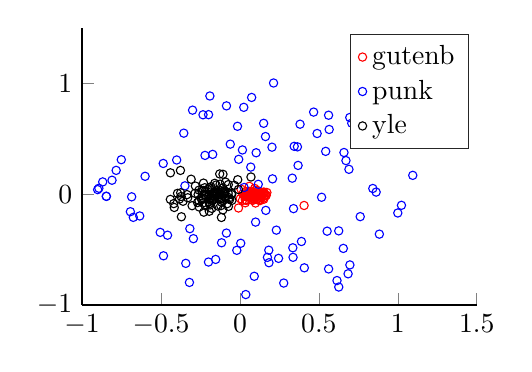
\begin{tikzpicture}

\begin{axis}[%
width=142.638pt,
height=100pt,
at={(0pt,0pt)},
scale only axis,
xmin=-1,
xmax=1.5,
ymin=-1,
ymax=1.5,
axis background/.style={fill=white},
axis x line*=bottom,
axis y line*=left,
legend style={legend cell align=left,align=left,draw=white!15!black}
]
\addplot[only marks,mark=o,mark options={},mark size=1.5000pt,color=red] plot table[row sep=crcr]{%
0.127320375358783	-0.0086918456764386\\
0.0957460994019254	0.0121368277749043\\
0.0890281678423096	0.00496880629574048\\
0.0998107221618694	0.0339405201907585\\
0.0290636608072532	-0.0156031300689192\\
0.147871166582909	0.0166552815660188\\
0.137370791106716	-0.00899786769326917\\
0.0459636949605271	-0.00418479912217206\\
0.148140548280657	-0.0355617122460245\\
0.113718988746527	0.00311104110429118\\
0.0628039791121674	-0.0280914774181388\\
0.12212771095968	-0.0255206536915069\\
0.167092318430627	-0.00774613067753573\\
0.103569317087268	-0.0180438871181655\\
0.0591985274469038	0.0716385972621419\\
0.12326037533193	-0.000903336092140371\\
0.00660716371053004	0.0462542937163954\\
0.0362452983809937	-0.053271956967899\\
0.0857103971649569	-0.0426038293395847\\
0.0387552301829534	0.0250307391160174\\
0.0179356949761165	0.0029586178839492\\
0.158350322090383	-0.00679416524844419\\
0.140581353704651	-0.00244871780614607\\
0.124524150041842	0.0123241358604416\\
0.0573463922253305	0.00983547710140347\\
0.0158563121614287	-0.0560986273212817\\
0.0976434011450581	-0.010418694592789\\
0.153157958994887	0.00678207048439472\\
0.0729934782578269	0.0121380931131039\\
0.130178651978624	0.0185607779027115\\
0.0568252713257679	-0.0069031545746218\\
0.0685822191116412	0.00811931675947374\\
0.111970190144691	-0.0114956699772057\\
0.0366345525878751	-0.0196291197820779\\
0.0668551201328866	-0.026641176419254\\
0.0908044240307837	-0.0452682061980333\\
0.0774523385183702	-0.00426940192338515\\
0.406323844794709	-0.101346134576406\\
0.0807063875819902	-0.0552793287701591\\
0.0398736305244038	-0.00438044346104674\\
0.0284952534249072	-0.0131646730145714\\
0.0656155880303887	-0.00682412744760175\\
0.0712516426966222	0.0169473541904283\\
0.129803402251114	-0.00359229701783019\\
0.0668383093755703	-0.0134307464403234\\
0.162937503756807	-0.0133468602947013\\
0.114428971109603	0.0319266978049882\\
0.0369901774631491	-0.0204952886956791\\
0.0021575365648745	-0.0403124723696447\\
0.0794091731751481	0.000591817800292282\\
0.0873481783577699	-0.0157537607231872\\
0.0439805382513202	0.00634358278087417\\
0.170572977856609	0.0160406164736429\\
0.0668182906292148	-0.00346446298599108\\
0.0450581714424684	-0.0185726873576098\\
0.065519127612359	-0.000895071514525758\\
0.0965591120859067	-0.00147075154469128\\
0.0597922197592608	-0.0262732653202667\\
0.0512766138049637	-0.0129682656960005\\
0.130639981495391	0.0138658473572791\\
0.0337350921888365	-0.0770750577702149\\
0.119416875315215	-0.0117275809345634\\
0.0548775805313886	-0.0141111861746138\\
0.12833109431344	-0.0564198971399988\\
0.0533240441983922	-0.00893951513430827\\
0.11906906193826	-0.0533836262284981\\
0.0930615791330474	0.0529922703181468\\
0.0697514190093523	-0.0134300117587801\\
0.0888821905323755	-0.0124567844382612\\
0.0914187304065824	-0.0178560927719924\\
0.0729092400284866	-0.00616598595881895\\
0.107305960174481	-0.0151368894697283\\
0.123842402012303	-0.0533154951534984\\
0.0853738958376601	-0.0352843713059079\\
0.0854635328804408	-0.0199393522813179\\
0.0584399198349393	0.00512924067782563\\
0.0616382476458653	0.0255819583955573\\
0.152052052127736	0.0201481362781212\\
0.151238583846108	-0.0447634357416128\\
0.0712854946345532	0.000698685738264215\\
0.0884661418712211	-0.00781470629828667\\
0.100292568824025	-0.0178084260914522\\
0.0435101039144675	0.00825160030788957\\
0.0986908882608514	-0.0790044672047437\\
0.0590765560557244	-0.00441352549651264\\
0.100593102504738	0.00576761109811074\\
-0.00905653855428984	-0.124134065514804\\
0.0724361615864486	-0.0461024273423489\\
0.103556742253584	-0.00743419521517522\\
0.105777253144801	-0.0430120918484251\\
0.0674868347468651	0.00299980600774744\\
0.0322227385898126	-0.00953304800145252\\
0.131496061165266	-0.0111962044749197\\
0.034382755316276	-0.0491637646908142\\
0.0753508356883622	0.0188285752918651\\
0.0423801349212037	-0.054319099449739\\
0.145708838477977	0.00613589247115466\\
0.104239757179167	0.012515237332608\\
0.0364144071893882	-0.00362746659379873\\
0.0852630708823695	0.00835495993217901\\
};
\addlegendentry{gutenb};

\addplot[only marks,mark=o,mark options={},mark size=1.5000pt,color=blue] plot table[row sep=crcr]{%
-0.90117977852833	0.0418863864839486\\
-0.675422916229891	-0.208544452425357\\
0.336385126204716	-0.569617626756744\\
1.09466163059029	0.170793599809734\\
-0.846089359018064	-0.0183598325725213\\
0.671575520465693	0.304382387813222\\
-0.693850554333806	-0.157549224987796\\
0.331452624097514	0.145339653677192\\
0.343704649531415	0.433166945928725\\
0.658931177487138	0.377223939588205\\
-0.317198941964371	-0.31058359881451\\
0.695739099376215	0.693375988195135\\
-0.893494058640877	0.0542730728436936\\
0.164001334529278	-0.145664422000098\\
0.389643917138755	-0.426696582237827\\
0.230724935613333	-0.324126570087027\\
-0.685763506226415	-0.0231110378212933\\
0.625916854583977	-0.837983706434924\\
-0.348257174865099	0.0762074441909927\\
0.0907782312273092	-0.741022408631092\\
0.244676666681733	-0.579024833301159\\
-0.355631918228014	0.552004619274315\\
-0.221099749506679	0.351028035252879\\
-0.190277469546502	0.88778273380042\\
0.466852459970199	0.742247238332434\\
0.561415679421435	0.714126258290433\\
0.708111581006574	0.642522697539496\\
0.182716160904971	-0.505390031030646\\
0.203054062184905	0.425296370464828\\
0.277365229497161	-0.802074216853215\\
0.862691169017095	0.0196216758713334\\
-0.294760452115802	-0.401125098340321\\
0.364240432757956	0.428443365566202\\
-0.0198956668321366	-0.5063826540231\\
0.0158973264455835	0.400297152578139\\
0.685013355681693	-0.718440766870158\\
0.183852326910061	-0.618293313270519\\
-0.116210409047691	-0.438145365672136\\
0.174195127357218	-0.569790025020028\\
-0.0612122232452297	0.452702707587755\\
0.841576872572119	0.0522062086598045\\
-0.153577799619812	-0.588523843621319\\
-0.783868382828821	0.215874768507118\\
-0.634607668276075	-0.195888978048004\\
0.54317136744375	0.387677766826667\\
0.150228439224951	0.641047592521172\\
-0.172546929601628	0.360219986748599\\
0.883034932365545	-0.360293644843348\\
-0.342899319336636	-0.624149077661272\\
0.745925778119947	0.623726934755658\\
-0.0153630999986672	0.614182061349798\\
0.488997036591371	0.548976952988982\\
1.02306184481199	-0.0998207705180281\\
0.625644021560171	-0.330502605570339\\
-0.400577381964277	0.309593248053915\\
-0.484161844489307	-0.555821474773981\\
0.074209683466211	0.874668206275771\\
-0.600574230061715	0.162395071809437\\
0.116143035669922	0.0898792193234591\\
0.552275711552865	-0.333474128606332\\
-0.810106284106562	0.126705497056851\\
0.614792998180342	-0.779679168055662\\
0.561648730523823	-0.674575039599506\\
0.212922423573955	1.0052048713606\\
-0.199243999431619	-0.612192472848048\\
0.690352132322671	0.225402320892353\\
0.334918470844195	-0.483358973706908\\
0.0992157447010421	-0.251509488788502\\
-0.0855889423257792	-0.350647698278089\\
-0.299956445714413	0.759769628854066\\
-0.504872357697814	-0.344289047901931\\
-0.00778525945542807	0.315579692816992\\
0.024394342459716	0.785309200629355\\
-0.2338734847162	0.718026967252166\\
-0.751350002755071	0.312394775818612\\
-0.198648040050147	0.719111622256081\\
0.56527960994794	0.585220204704732\\
0.0050302940616785	-0.442772292398161\\
0.654821345236676	-0.489120893108261\\
0.0371878108167786	-0.905953128777966\\
0.102896925963496	0.374938560651166\\
-0.846064463194802	-0.018388721824942\\
0.380752716676433	0.632919096094651\\
0.02644081555163	0.061264615367709\\
0.0685934007440231	0.245419661789938\\
-0.458422970148582	-0.369815452110831\\
0.769836349061794	0.52467574255742\\
-0.31981983359287	-0.796489192759173\\
-0.48584354415051	0.278250363169434\\
-0.869168427870437	0.111605648747747\\
0.161925615085964	0.521463588879641\\
0.339379327585913	-0.129720606320129\\
0.696412568871254	-0.638336691802383\\
-0.0851925860775196	0.798674369162145\\
0.517267362832254	-0.0270608899438363\\
0.999816602335205	-0.169029888047282\\
0.206441832556375	0.139228974513592\\
0.761870246793029	-0.202046022689163\\
0.407834371777991	-0.664477826560396\\
0.368316878313544	0.260609751838578\\
};
\addlegendentry{punk};

\addplot[only marks,mark=o,mark options={},mark size=1.5000pt,color=black] plot table[row sep=crcr]{%
-0.0961448175034892	0.00364637121813632\\
-0.122476234695974	-0.0279715812984106\\
-0.171676584447112	0.00832971605028357\\
-0.185931689650042	-0.0321044231032855\\
-0.187274445115069	0.0197104828843733\\
-0.202740045304088	0.0429440014004054\\
-0.156146143972949	-0.00771120119469056\\
-0.0509761676797131	-0.0551534483821851\\
-0.108134045612394	0.0573153256146896\\
-0.0527460839882873	0.00775409794530984\\
-0.360314751955368	-0.063332846912988\\
-0.074955439517982	0.0109451709531295\\
-0.230500129124114	-0.0357170921505507\\
-0.0951037924912044	0.0280987440348195\\
-0.159665996775884	0.0989283261242778\\
-0.118094002524702	-0.0404636955607253\\
-0.268637797691877	-0.0749005884309451\\
-0.0912603053475185	0.109411373182182\\
-0.37242944539053	-0.0200709171274847\\
-0.0138232437156533	0.131455619756612\\
-0.176937986894496	-0.0117073952667855\\
-0.258945217271117	-0.0592361756596638\\
-0.184061571532035	0.0676211476467834\\
-0.41914020427523	-0.0841598393362775\\
-0.188868740037633	-0.0964448292732849\\
-0.0914906489789569	-0.0343845921196073\\
-0.24030146472312	0.0241781710626134\\
-0.33499591592017	-0.00312139225188903\\
-0.178231394650282	-0.127558867003038\\
-0.109760834966189	0.0248788445741339\\
-0.128101135129127	0.183565278288583\\
-0.440235220537448	0.193772070432993\\
-0.194269468327805	-0.153512254733672\\
-0.259101255081798	0.0373705024681628\\
-0.0814885376521595	-0.0856739163610967\\
-0.370668482186611	-0.203323175371792\\
-0.416032681866337	-0.11925229458215\\
-0.121245968919095	-0.103329152387799\\
-0.12427124955257	-0.00302263860789706\\
-0.169198963646184	-0.0155881428612704\\
-0.282022961567763	0.0741770240059802\\
-0.0968600188499422	-0.0189652705235905\\
-0.0674234252272486	-0.0319752491959172\\
-0.240211819562252	-0.048458565996857\\
-0.179067751470528	0.0518571776314357\\
-0.108271795695194	-0.141170180507986\\
-0.223019661403637	0.0589410111951817\\
-0.194356316154312	0.0568316302328363\\
-0.139417533019799	-0.0257970130366122\\
-0.440641610109931	-0.0466311620728764\\
-0.132583108595895	-0.00381611151292361\\
-0.214819422773987	-0.010952065985742\\
-0.125835212159475	0.0912952388017828\\
-0.395208384798469	0.00832371946648758\\
-0.0730606613372144	-0.110120738571015\\
-0.177026498217943	-0.0534382725659169\\
-0.125854894703434	0.0349565343657289\\
0.0700249434059015	0.156068548631834\\
-0.230792057379853	0.100618903910244\\
-0.14694382965944	0.0173887670032555\\
-0.309155222375835	0.135865089037344\\
-0.139679334553703	-0.106329817694199\\
-0.219491402464095	-0.104296133309745\\
-0.192682182152125	-0.0822546644168206\\
-0.173652788494436	-0.0566005010916457\\
-0.00943990716889307	0.04309142980815\\
-0.18444180186741	-0.0395096214606103\\
-0.0735505169193182	0.0869708113641472\\
-0.116566776370826	-0.0709366340007293\\
-0.10236186418912	0.0147887110621152\\
-0.194666559953024	-0.000668384893972641\\
-0.15069567186011	0.0834992241786669\\
-0.113843614777405	-0.055296702081269\\
-0.169039460487251	-0.0364702744223241\\
-0.234637290911474	-0.0787830813079343\\
-0.0526147744130464	-0.00314867954784847\\
-0.284277474014985	0.00848947983717682\\
-0.244612050044909	-0.0384341760115537\\
-0.154944978618333	0.0138989513525338\\
-0.302887161027531	-0.103359681221306\\
-0.330527976757136	-0.0314348460537532\\
-0.0966701651204119	0.0159078718421593\\
-0.382761124712952	-0.0431048733570848\\
-0.194978563983009	-0.0681551484024036\\
-0.257826606045121	-0.115170463171982\\
-0.169739899158024	-0.0476551759019462\\
-0.129139391016185	0.00216274342037229\\
-0.156346206578657	-0.00223507823749834\\
-0.107325465101006	0.180400287685329\\
-0.264542576382817	-0.00179840645549771\\
-0.168603547640312	0.0112963211564749\\
-0.225616665711826	-0.000475192944848947\\
-0.228819601252936	-0.161528945203531\\
-0.230717448263335	0.0341742079876436\\
-0.375209363760451	0.0131736869555462\\
-0.11717735053545	-0.209447872977298\\
-0.144751603782121	0.00783024318528655\\
-0.0354900220019975	0.0808385607492133\\
-0.376741073281636	0.215434565623507\\
-0.0649596425411832	-0.0463757177430812\\
};
\addlegendentry{yle};

\end{axis}
\end{tikzpicture}%
    \end{column}
  \end{columns}
\end{frame}

\begin{frame}
  \frametitle{Exploration - clutering on trigrams}

\end{frame}

\begin{frame}
  \frametitle{Ideas for exploitation}
  \begin{itemize}
    \item Original aim is to obtain a metric\pause{}

    \item But this is an unsupervised situation (unless we make assumptions
      about the different sources as class labels) so simple regression is not
      possible\pause{}

    \item If we can identify separate classes and characterise them with a
      metric, unseen data can be characterised by taking a weighted sum\pause{}

    \item More sophisticated extensions might be possible, eg Guassian mixture
      models trained with expectation maximisation would consider different
      clusters to have different amounts of spread.
  \end{itemize}
\end{frame}

\begin{frame}
  \frametitle{Potential future work}
  \begin{itemize}
    \item TD-IDF.\pause{}

    \item Use segementation to enable a ``bag of morphs'' model. Useful
      since eg -ni, -si, -mme, -tte strongly suggest written language.\pause{}

    \item Obtain a supervised data set.
  \end{itemize}
\end{frame}

\end{document}
